\documentclass[11pt]{article}
    \usepackage{amsmath}
    \usepackage{graphicx}
    \usepackage{color}
    \usepackage{longtable}
    \usepackage{tabu} %% text tables
    %%\usepackage[linktocpage=true]{hyperref} %% links to numbers instead of sections
    \usepackage{hyperref}
    %%\usepackage{url}
    \usepackage{geometry}
    \geometry{left=1.5cm,right=1.5cm,top=1.5cm,bottom=1.5cm}
    \graphicspath{{./images/}}
    \usepackage{amsmath}
    \usepackage{amssymb}
    \usepackage{calc}
    \usepackage{ifthen}
    \usepackage{tikz}
    \usepackage{svg}
    \usepackage{float}
    %%\usepackage{cite} 
    %%\usepackage{notoccite}
    \usepackage[backend=bibtex,sorting=none]{biblatex}
    \addbibresource{seedom.bib}
    \renewcommand*\rmdefault{ppl}
    \setlength{\fboxsep}{10pt}
    \setlength{\fboxrule}{0.5pt}

\begin{document}

\title{%
\Huge Seedom \\[4mm]
\large Timely \& Relevant Charity Fundraiser \\[1mm]
with Supporter Rewards}
\author{Team Palm Tree}
\date{\today}
\maketitle

\begin{abstract}
There isn't an efficient, transparent, and trustless method to facilitate positive charitable organizations and the members of society they serve in a time of crisis. Fundraisers take time to put together and crowd-sourced campaigns often lack transparency and have to spread through word-of-mouth. Seedom is a fundraising and supporter rewards platform that allows anyone to seed fund trustworthy charities that deal directly with afflicted individuals in a trustless fashion, thereby augmenting these individuals' freedom in an otherwise oppressive world. Bimonthly, a new timely and relevant charity will be chosen to receive about half of the funds raised through our smart contract. The other half of the funds will go towards one of the supporters, as selected by the participants at large along with the charity. A small percentage will be taken by the Seedom team as an administration fee in order to continuously improve this product through several phases, advertise with the charity, and celebrate the community-chosen participant.
\end{abstract}
\pagebreak

\tableofcontents
\pagebreak

\section{Introduction}

Seedom is an Ethereum decentralized application for raising awareness and funds for charities in need while rewarding a single supporting participant for their funds contribution. The selection of the winning participant is crowd-sourced from the participants and the selected charity. Funds raised will be distributed according to table \ref{tab:fundSplitPercentages}. Administration fees cover our expenses in four operational areas.

\begin{itemize}
\item{\textbf{Staff} team members, which include the president, founders, software developers, and the marketing team}
\item{\textbf{Legal} legal representation to protect private fundraising rights internationally}
\item{\textbf{Audits} continuous security and financial audits as organizational and technological changes are made}
\item{\textbf{Events} additional physical fundraisers to further raise money for and promote charities}
\end{itemize}

\begin{table}[H]
\begin{center}
\begin{tabular}{| l | l | l |}
\hline
\textbf{Charity} & \textbf{Winner} & \textbf{Seedom} \\ \hline
47.5\% & 47.5\%  & 5\% \\ \hline
\end{tabular}
\caption{Fund split percentages}
\label{tab:fundSplitPercentages}
\end{center}
\end{table}

\subsection{Charity Selection}

Well before a fundraiser begins, the Seedom team will accept suggestions from various communication sources including email, text messages, chat app messages, and posts to our social media accounts. For phase one, the Seedom team will be the authority for charity selection. A charity will be chosen using several criteria.

\begin{itemize}
\item{\textbf{Legitimacy} the charity must be a non-profit with a proven record of benefitting the general public}
\item{\textbf{Relevancy} the charity must be working on a cause that is currently relevant}
\item{\textbf{Timeliness} their should be an urgent or ongoing need by the charity for assistance}
\item{\textbf{Cooperative} the charity must be willing to work with the Seedom team}
\end{itemize}

\subsection{Combination of Qualities}

Seedom is the first fund raising and rewards platform with all of the following qualities.

\begin{itemize}
\item{\textbf{Philanthropic} a new excellent charity will be chosen bimonthly}
\item{\textbf{Trustless} trust in the charity is all that is required}
\item{\textbf{Transparent} all contract transactions publicly visible and immutable}
\item{\textbf{Relevant} legitimate charities working on focused causes that have an ongoing need for assistance }
\item{\textbf{Secure} security is provided by the Ethereum platform itself and MetaMask}
\item{\textbf{Anonymous} a wallet is the only requirement
\item{\textbf{Private} any identifying information given is purged after each fundraiser}
\item{\textbf{Global} anyone in the world can participate}
\item{\textbf{Affordable} everyone will be able to afford an entry}
\item{\textbf{Limitless} there is no limit to the number of entries that can be obtained}
\item{\textbf{Instantaneous} payouts to the charity and the winning participant are immediate after the fundraiser ends}
\end{itemize}

\subsection{Comparison to Other Fundraising Methods}

Many methods exist for raising funds for charities. Outside of direct donations, some of the most popular include crowdfunding, matching gifts, drives, sales, auctions, events, lotteries, and raffles. All of these methods lack many of our combined qualities.

\subsubsection{Crowdfunding}

Crowdfunding is one of the best ways to raise funds for a charity or cause. Unfortunately, most of the popular fundraising platforms are not on Ethereum and therefore receive none of the many benefits native to the platform. When using a centralized website, such as GoFundMe, one is relying on them as to move funds from donors to a charity. Without trustless transaction transparency, it is impossible to know if these funds ever made it to their destination. Moreover, many crowdfunding companies charge 8+\% fees for any donation, which includes a hefty payment processing fee. Because of this reliance on payment processors, GoFundMe is only available in a handful of counties.

\subsubsection{Matching, Drives, Sales, and Auctions}

Matching, drives, sales, and auctions are also effective fundraising vehicles. Donation matching requires one to work for or know a company that offers this perk. Donation drives may involve an intermediary that converts physical donations into monetary ones. Sales of items require the overhead of procuring items to sell in addition to the resale activity. Auctions items must be solicited, hopefully for free, and then sold for donation funds. Because of the various requirements and overheads involved with each of these techniques, the timeliness and relevancy of the ultimate donations might be lacking and with middlemen involved, trust and transparency are still huge issues. All three of these also lack global participation.

\subsubsection{Events}

Fundraising events are social gatherings that raise funds and awareness for a charity. Face to face communication is indispensable to furthering a cause and should never be overlooked. However, events can get expensive when selecting a venue, hiring temporary staff, providing food, creating informative materials, etc. Seedom adopts this technique at the end of each fundraiser for the mentioned benefits in addition to celebrating the newfound success of the winning supporter. In this way, the bulk of the funds have already been raised and distributed, making this final event important, but not necessary to the success of the chosen charity.

\subsubsection{Lotteries \& Raffles}

Although Seedom is not a lottery and not a raffle, similar organizations exist worldwide and all of them have administration fees for their existence. In the United States, nearly every state has its own lottery, with a national average administration fee of 4.76\% according the the U.S. Census Bureau \cite{3}; however, this does not include commissions paid out to lottery ticket sellers, which equal this same percentage, on average \cite{4}. All expenses considered, 8-10\% of every lottery ticket sold in the U.S. goes towards the lottery process itself and not the winner(s) and beneficiaries.

\section{The Bimonthly Trustless Fundraiser}

Seedom will kickoff a new fundraiser for a new charity bimonthly, or roughly every two weeks, on the 1st and 15th of every month. Thirteen days is the span of the entire timeline due to February's 28 total days during standard years. Seedom will go on break on the 13th and 14th of every month in addition to the 29th until the end of any month long enough.

\begin{figure}[H]
\begin{center}
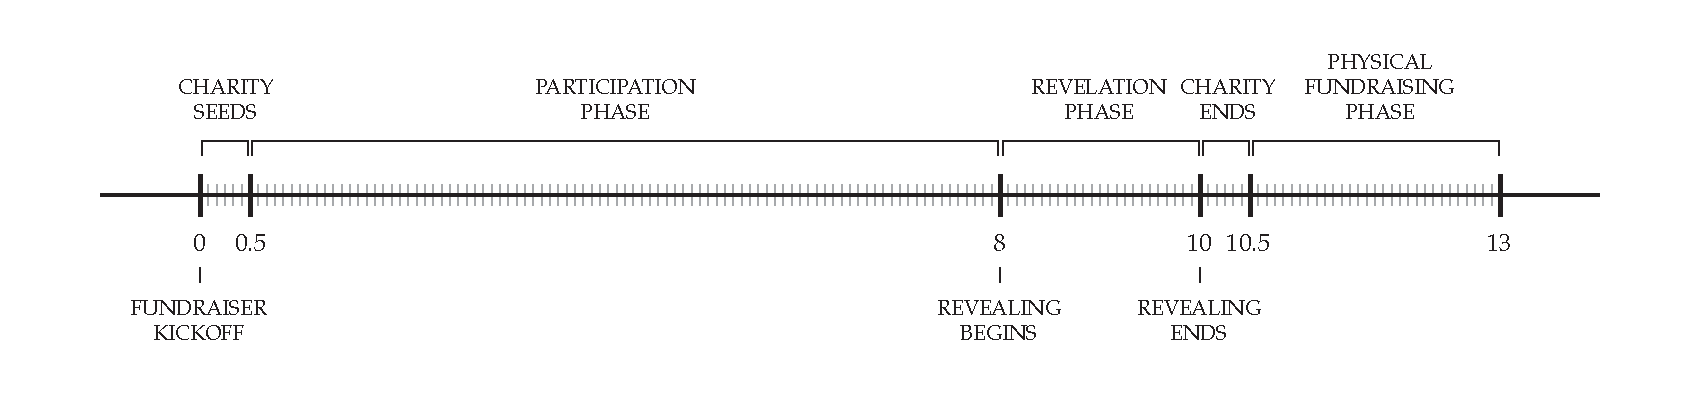
\includegraphics[width=1.0\textwidth]{fundraiserBimonthlyTimeline.pdf}
\caption{Fundraiser bimonthly timeline}
\label{figure:fundraiserBimonthlyTimeline}
\end{center}
\end{figure}

\subsection{Fundraiser Kickoff}
A fundraiser begins with the Seedom team kicking it off through our smart contract by providing several parameters defined in table \ref{tab:fundraiserKickoffParameters}.

\begin{table}[H]
\begin{center}
\begin{tabular}{| l | l | l |}
\hline
\textbf{Parameter} & \textbf{Data type} & \textbf{Description} \\ \hline
charity & address & the ethereum wallet address of the charity \\ \hline
charitySplit & uint256 & the \% of funds given to the charity \\ \hline
winnerSplit & uint256 & the \% of funds given to the winner \\ \hline
ownerSplit & uint256 & the \% of funds given to the owner \\ \hline
valuePerEntry & uint256 & unix timestamp of the start of revelation phase \\ \hline
revealTime & uint256 & unix timestamp of the end of revelation phase \\ \hline
expireTime & uint256 & unix timestamp of the expiration of the fundraiser \\ \hline
\end{tabular}
\caption{Fundraiser kickoff parameters}
\label{tab:fundraiserKickoffParameters}
\end{center}
\end{table}

\subsection{Charity Seeds}
Shortly after kickoff, the charity must create a 32-byte random number. This hashed random, the address of the charity's wallet, and the address of the active Seedom contract will be posted by the charity and Seedom through our respective social media accounts to guarantee their origin and authenticity. Any user can validate these pieces of data against the contract address state.

The charity will now seed the charity a 32-byte hash of it. Only the charity can provide this hashed number and no one can participate if it is not provided. All hashed randoms are generated using the hashed random formula in figure \ref{figure:hashedRandomNumberFormula}. The charity must safeguard their random number and not reveal it to anyone outside of their organization. It will be used later when the charity ends the fundraiser. If the charity does not seed the fundraiser before the revelation phase, the fundraiser is a dud and all participants will be refunded upon cancellation.

\begin{figure}[H]
\begin{center}
\fbox{$hashedRandomNumber = sha3_{keccak256}(randomNumber, ethereumAddress)$}
\caption{Hashed random number formula (randomNumber is 32 bytes, ethereumAddress is 20 bytes)}
\label{figure:hashedRandomNumberFormula}
\end{center}
\end{figure}

\subsection{Participation Phase}

After the charity has submitted their hashed random number, the fundraiser is considered open and anyone can now participate and send ether to the contract. Participation is a one-time activity and first, a user must create their own 32-byte random number and hash it using the formula in figure \ref{figure:hashedRandomNumberFormula}. The user must safeguard their random number and not reveal anyone else. It will be used during the revelation phase to confirm their participation in the fundraiser. The participation function also accepts ether funding to obtain entries.

Each entry costs a fixed value determined by the Seedom team at kickoff. The cost of a single entry will be very affordable to those beneath the international poverty line of \$1.90 (USD) per day\cite{1}. Each entry increases the likelihood that you will be selected by both the community and the charity to receive a split percentage of all of the ether received by the contract, similar to a raffle. If you are the winner of this ether, you will also be invited to participate in the physical fundraiser event after the end. Entries cannot be refunded and must be confirmed during the revelation phase. Partial entries will be refunded immediately when participating or through additional funding after participation. The owner and the charity are never allowed to participate.

Along with the hashed random and any ether, a user can optionally associate their Ethereum address with a short alias and their email address. These three values are stored off-chain in Seedom's secure servers and are forgotten by the time the next fundraiser begins to protect user privacy and keep our system GDPR compliant. For phase one, the alias is used to render a list of recent participants. The email address is only used to invite the community-chosen winning supporter to the physical fundraiser during the last few days.

After initial participation, more ether can be sent to the smart contract directly to obtain more entries. However, additional calls to participate will fail and the participant's hashed random number cannot be altered. There are no limits to the numbers of entries a participant can obtain and the participant can check the number of entries they or any other participant have through the contract at any time.

\subsection{Revelation Phase}

When the revelation phase begins, calls to participate and fund will fail. Participants may now reveal their secret random numbers, sent hashed in the participation phase, to the rest of the community. All random numbers need not be revealed; however, failing to reveal a random number will result in the forfeiture of funds without the ability to win community selection. Successful revelations may only be performed once per participant and incorrect random revelations, determined using the formula in \ref{figure:hashedRandomNumberFormula}, will be rejected.

\subsection{Charity Ends}

When the revelation phase ends, participants are no longer allowed to reveal their randoms. Between the end time and expire time, both specified during kickoff, the charity must now reveal their random number provided during seed. If the charity fails to call the end function and reveal their random before the expire time, all entries can be refunded through cancellation.

\subsubsection{Secure Deterministic Crowd-sourced Random Number Generation}

Because Ethereum is a turing complete deterministic world computer, mining nodes cannot generate individual random numbers as they would never be able to reach consensus. Some decentralized applications decide to use a miner-defined value, such as the blockhash, timestamp, or other value to generate a random number. This technique is flawed because of this and the miner's ability to reorder transactions, not include transactions, and not send out blocks. This gives the miner additional chances of winning.

Seedom's technique in similar to that of the RANDAO\cite{2}. It starts with a hashed random seed provided by the charity, a collection of secret hashed randoms in the participation phase, and the revelation of these randoms during the revelation phase. All of these revealed random numbers are XORed together, starting with the participant randoms and ending with the charity random, to produce a final universal crowd-sourced random that will be used to determine the winning participant, as seen in figure \ref{figure:crowdsourcedRandomNumberGeneration}.

\begin{figure}[H]
\begin{center}
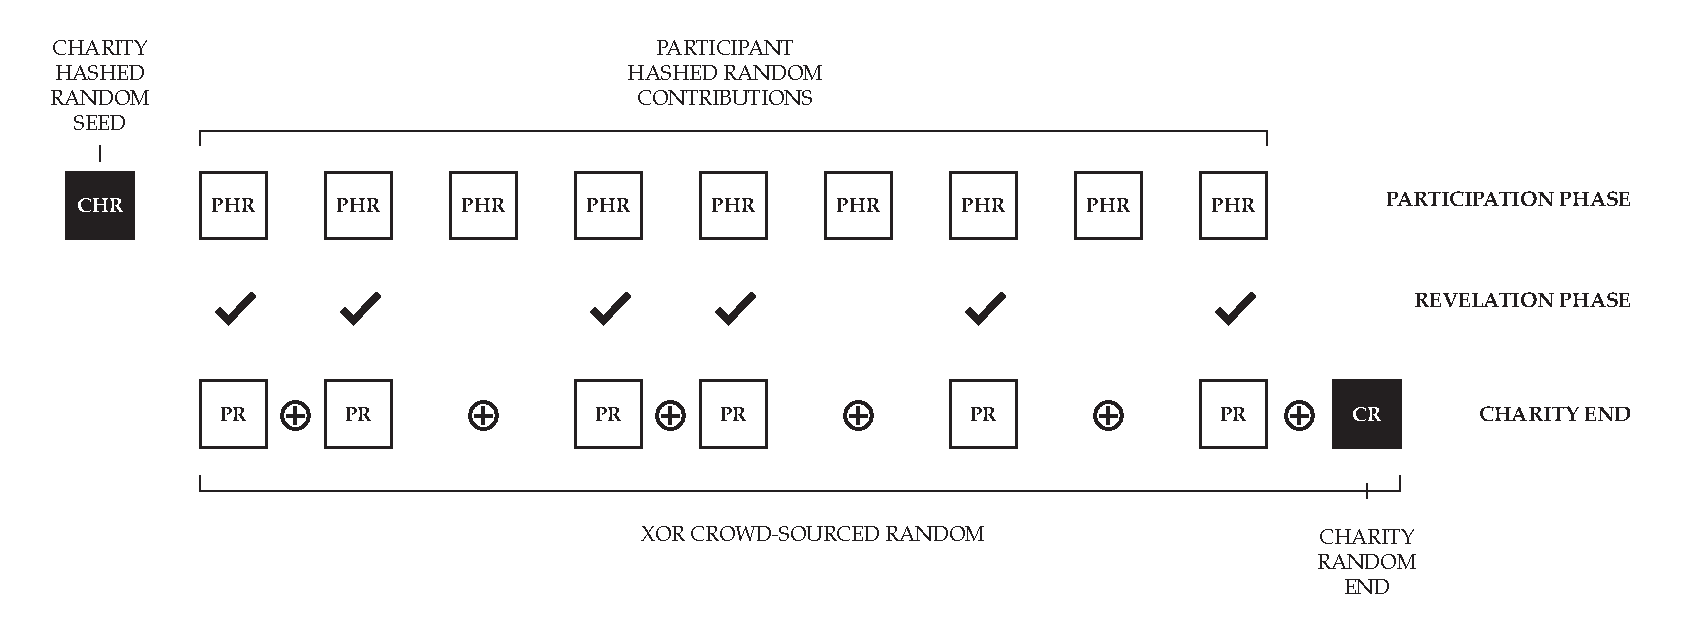
\includegraphics[width=1.0\textwidth]{crowdsourcedRandomNumberGeneration.pdf}
\caption{Crowd-sourced random number generation}
\label{figure:crowdsourcedRandomNumberGeneration}
\end{center}
\end{figure}

If hashed randoms are only collected and revealed from the participants, the last participant has the choice to reveal their random, essentially giving them a double chance of winning. Worse yet, a miner that has participated many times using unique wallet addresses can gain many additional chances by reordering their reveal transactions and choosing which ones to publish. Because the cost of a Seedom entry will be low enough to be affordable by all, transaction gas and entry costs will not deincentivize bad miners from using this method.

To prevent this kind of tampering by the miners, the charity must be used as a trusted third party to provide a random that can alter any manipulation by miners. This charity random is provided hashed before the first user participates so that the charity cannot themselves manipulate the final crowd-sourced random. Users participating in a fundraiser tied to a specific charity are confirming their trust of the charity and their beneficial work. This trust extends to the charity's ability to seed start the fundraiser with their hashed random and end it with their final random revelation. The charity is incentivized to start and end a fundraiser because of the ether they will receive.

\subsubsection{Winning Participant Selection}

After the crowd-sourced random number is generated as part of the end call from the charity, it will be modded with the total number of revealed entries to determine an index into the global pool of revealed entries. A discrete cumulative density function is generated to assist with this process. density function The participant associated with the entry at this index is the winning supporter. As a last step in this call, a balance mapping is updated with owed funds to the charity, winner, and owner. Ether is not immediately distributed to each individual to prevent invalid or malignant addresses from reverting the end call. A winner is always guaranteed during each and every bimonthly fundraiser.

\begin{figure}[H]
\begin{center}
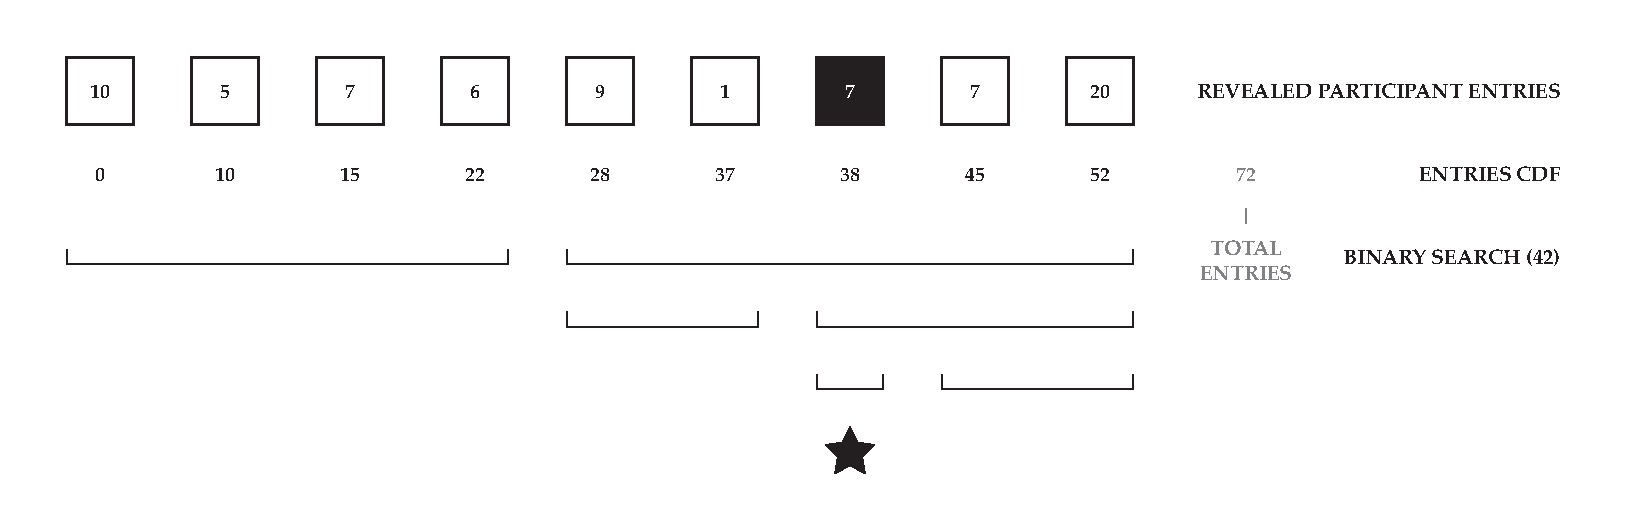
\includegraphics[width=1.0\textwidth]{winningParticipantSelection.pdf}
\caption{Winning participant selection for entry index 42}
\label{figure:winningParticipantSelection}
\end{center}
\end{figure}

\subsection{Physical Fundraising Phase}

After the end function completes, the charity, winner participant, and the owner can now withdraw their funds by calling the withdraw function. These funds will be available for withdraw at any time and will never expire. As a best practice, it is recommended that everyone withdraw their funds as soon as possible.

Now that the Ethereum fundraiser is over, a physical fundraiser will take place near the headquarters of the benefitting charity to celebrate their success. The winning supporter will be invited by email, if provided to Seedom, to an all expenses paid trip to this event, wherever it may be in the world. Seedom will provide staff to work with the charity to throw this final fundraiser. Afterwards, this process begins again.

\subsection{Fundraiser Cancellation}

At any time after kickoff and before end, both the charity and the owner can cancel the fundraiser. Cancellation is a simple process in which all entries are refunded to the respective participant addresses. This is done by updating the same balances mapping used to distribute charity, winners, and owner funds. After cancellation is complete, users may withdraw their refunds using the withdraw function. Gas costs cannot be refunded.

After the charity issues the end call, cancellation is impossible as funds have already been appropriated into the balances mapping. However, if the charity fails to end a fundraiser before the expire time, the cancel function becomes open to the charity, the owner, and the community. This ensures that even if something catastrophic happens to the owner and the charity, all entries can be refunded.

\section{Token Sale}
Never.

\section{Future Work}

\subsection{Ordered Statistic Tree Participant Storage}

\subsubsection{Participants Leaderboard}

\subsubsection{Entry Numbers}

\subsection{Handling Fund Growth}

As Seedom's participant base grows, our administration fee and winner selection process may need to be altered.

\subsubsection{Administration Fee Reduction}

Starting at 5\%, our administration fee should be adequate to maintain our decentralized application and protect this idea from any legal involvements that may arise. There are many laws and organizations spanning the local, country, and international jurisdictions that might impede the creation of a fully transparent and trustless private international fundraiser of this magnitude. As those concerns are abated, our administration fee will likely be reduced, at our discretion, to ensure maximal returns to the charity and our community. The administration fee will never be set above 5\%.

\subsubsection{Multiple Winning Participants}

There is an inherent burden that comes with the large influx of funds to any individual. Therefore, as the fund gets larger, we may introduce, at our discretion, the ability for multiple winners. Each successive winner might receive more funds than the last or a pool of winners may equally split the funds. There will only be one benefitting charity for any fundraiser, however.

\subsection{Crowd-sourced Charity Selection}

\section{Team Members}
\vbox{
\begin{itemize}
\item{\href{https://www.linkedin.com/in/jesse-kuiper-cpa-771a2111}{Jesse Kuiper}, Founder \& President}
\item{\href{https://www.linkedin.com/in/awgneo}{Alex Groleau}, Founder \& Software Developer}
\item{\href{https://www.facebook.com/eric.l.m.thomas}{Eric Thomas}, Software Developer}
\item{\href{https://www.linkedin.com/in/kylegraden}{Kyle Graden}, Marketing Lead}
\end{itemize}}

\pagebreak

\printbibliography

\vspace*{\fill}

\begin{flushright}

\pdfcreationdate
\end{flushright}
\end{document}